\begin{vbframe}{Example Practical Method}
Given: 20 training observations, 12 negative and 8 positive

\vspace{20pt}

\tiny
\begin{tabular}{l|p{0.1cm}|p{0.1cm}|p{0.1cm}|p{0.1cm}|p{0.1cm}|p{0.1cm}|p{0.1cm}|p{0.1cm}|p{0.1cm}|p{0.1cm}|p{0.1cm}|p{0.1cm}|p{0.1cm}|p{0.1cm}|p{0.1cm}|p{0.1cm}|p{0.1cm}|p{0.1cm}|p{0.1cm}|p{0.1cm}}

  \hspace{-8pt} \#&  1& 2&  3&  4&  5&  6&  7&  8&  9& 10& 11& 12& 13& 14& 15& 16& 17& 18& 19& 20 \\ \hline
  \hspace{-8pt} C & N & N & N & N & N & N & N & N & N & N & N & N & P & P & P & P & P & P & P & P \\ \hline
  \hspace{-8pt} Score & .18 & .24 &  .32 & .33 & .4 & .53 & .58 & .59 & .6 & .7 & .75 & .85 & .52 & .72 & .73 & .79 & .82 & .88 & .9 &.92
\end{tabular}
\normalsize

\vspace{20pt}
$\Rightarrow$ sort by score and draw the curves:
\vspace{20pt}

\tiny
\begin{tabular}{l|p{0.1cm}|p{0.1cm}|p{0.1cm}|p{0.1cm}|p{0.1cm}|p{0.1cm}|p{0.1cm}|p{0.1cm}|p{0.1cm}|p{0.1cm}|p{0.1cm}|p{0.1cm}|p{0.1cm}|p{0.1cm}|p{0.1cm}|p{0.1cm}|p{0.1cm}|p{0.1cm}|p{0.1cm}|p{0.1cm}}

  \hspace{-8pt} \#&  20& 19&  18&  12&  17&  16&  11&  15&  14& 10& 9& 8& 7& 6& 13& 5& 4& 3& 2& 1 \\ \hline
  \hspace{-8pt} C & P & P & P & N & P & P & N & P & P & N & N & N & N & N & P & N & N & N & N & N \\ \hline
  \hspace{-8pt} Score & .92 & .9 &  .88 & .85 & .82 & .79 & .75 & .73 & .72 & .7 & .6 & .59 & .58 & .53 & .52 & .4 & .33 & .32 & .24 &.18
\end{tabular}
\normalsize
\end{vbframe}


\begin{vbframe}{Example Practical Method}
\begin{center}
\includegraphics[width=0.75\textwidth]{figure_man/roc-curve-ex2.png}
\end{center}
\begin{itemize}
  \item Best accuracy achieved with observation \# 18.
  \item Setting $\theta = 0.88 \Rightarrow$ accuracy of $15/20 \; \hat{=} \; 75 \%$.
\end{itemize}
\end{vbframe}



\begin{vbframe}{Explanation Mann-Whitney-U Test}
\begin{itemize}
\item First we plot the ranks of all the scores as a stack of horizontal bars, and color them by the labels.
\item Stack the green bars on top of one another, and slide them horizontally as needed to get a nice even stairstep on the right edge (See: practical method example for ROC curves):
\end{itemize}
\begin{center}
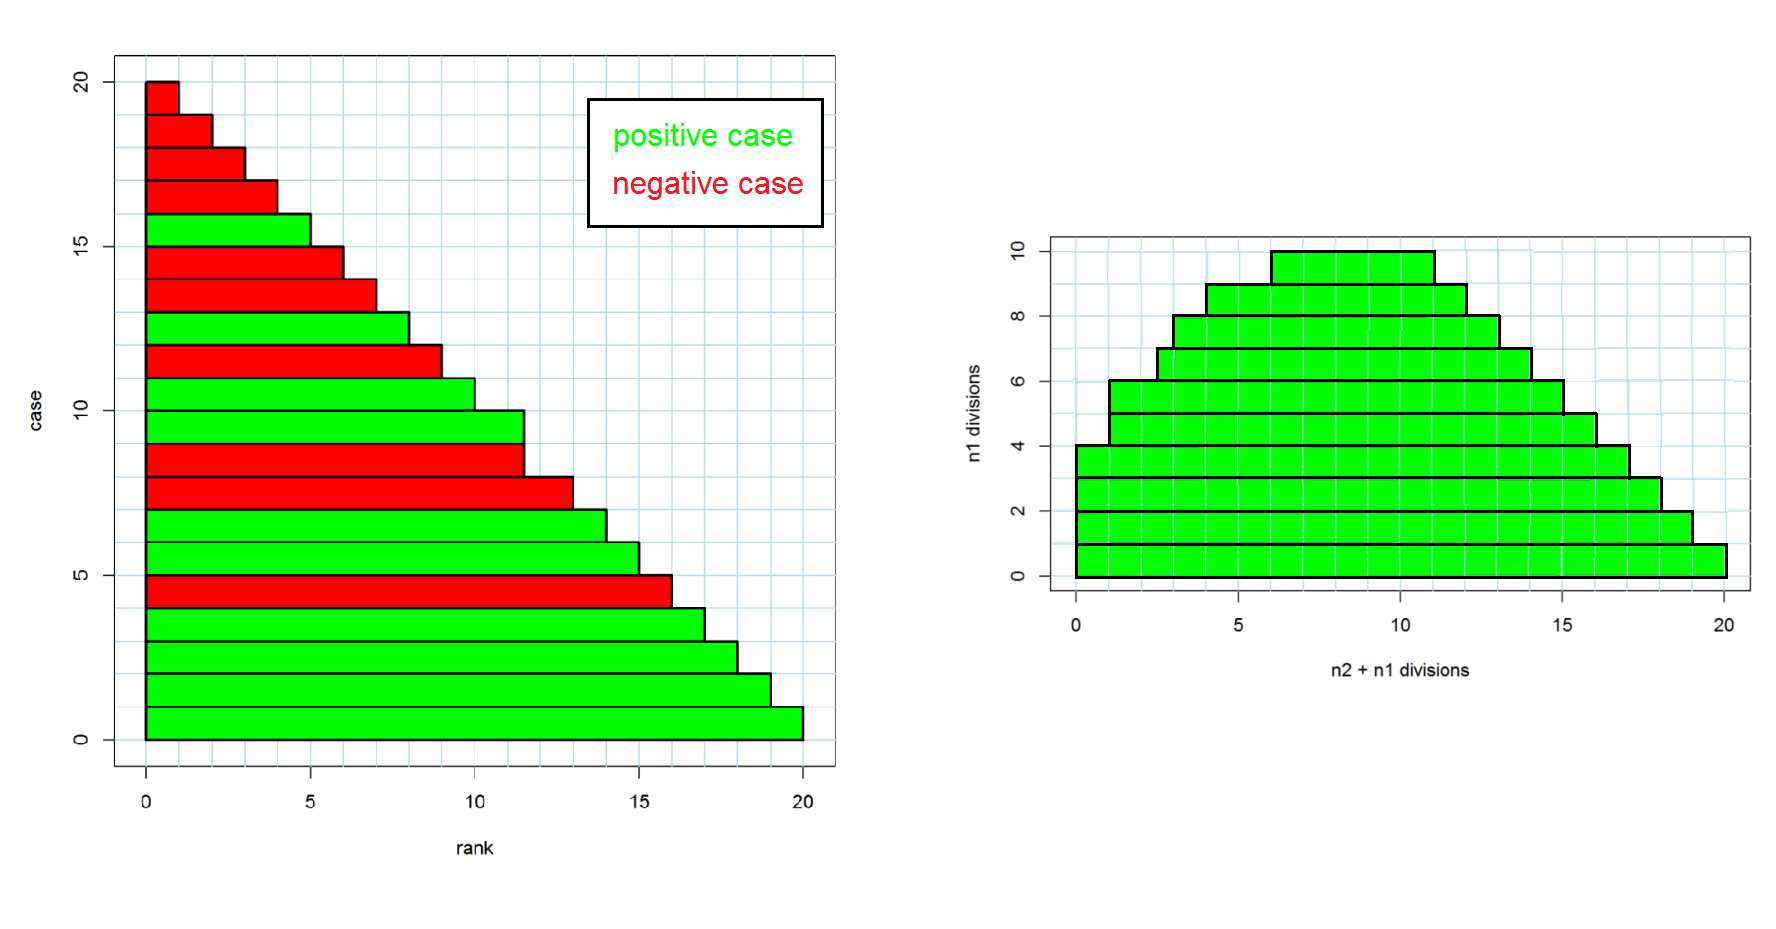
\includegraphics[width=0.8\textwidth]{figure_man/roc-mannwhitney3.png}
\end{center}


\framebreak


\begin{center}
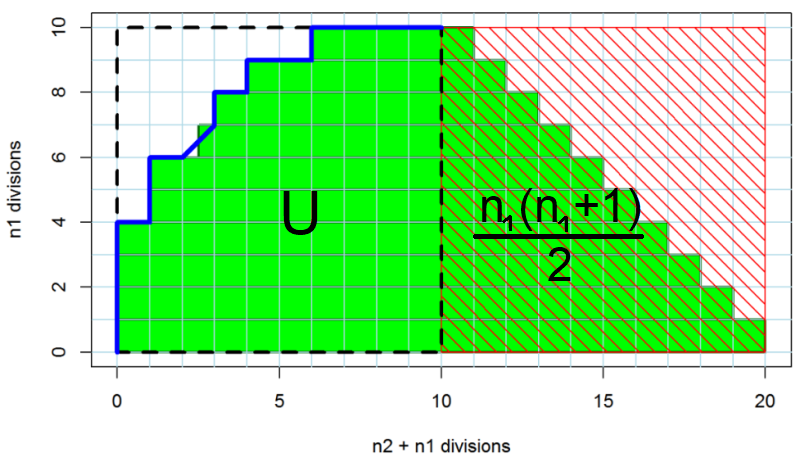
\includegraphics[width=0.5\textwidth]{figure_man/roc-mannwhitney2.png}
\end{center}

\begin{itemize}
 \item Definition of the U statistic: $U = R_1 - \cfrac{n_1(n_1 + 1)}{2}$
 \begin{itemize}
  \item $R_1$ is the sum of ranks of positive cases (the area of the green bars)
  \item $n_1$ is the number of positive cases
 \end{itemize}
  \item The area of the green bars on the right side is equal to $\cfrac{n_1(n_1 + 1)}{2}$.
\end{itemize}

\framebreak
\begin{center}
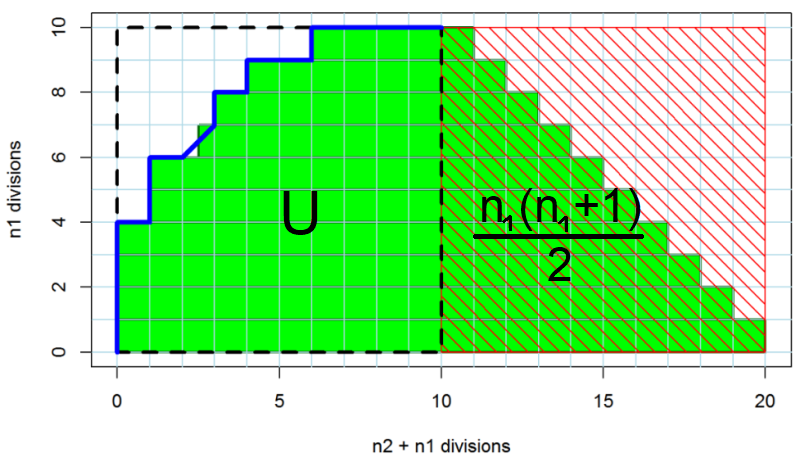
\includegraphics[width=0.5\textwidth]{figure_man/roc-mannwhitney2.png}
\end{center}

\begin{itemize}
 \item $U =$ area of the green bars on left side
 \item area of dashed rectangle = $n_1 \cdot n_2$
 \item $AUC$ is $U$ normalized to the unit square,
\end{itemize}
$$\Longrightarrow AUC = \cfrac{U}{n_1\cdot n_2}$$
with $n_1 = \text{POS}$ and $n_2 = \text{NEG}$.
\end{vbframe}


\begin{vbframe}{Partial AUC}
\begin{itemize}
  \item Sometimes it can be useful to look at a \href{http://journals.sagepub.com/doi/pdf/10.1177/0272989X8900900307}{specific region under the ROC curve}  $\Rightarrow$ partial AUC (pAUC).
  \item Let $0 \leq c_1 < c_2 \leq 1$ define a region.
  \item For example, one could focus on a region with low fpr ($c_1 = 0, c_2 = 0.2$) or a region with high tpr ($c_1 = 0.8, c_2 = 1$):
\end{itemize}



\framebreak

\begin{itemize}
  \item $\text{pAUC} \in [0, c_2 - c_1]$.
  \item The partial AUC can be corrected (see \href{http://journals.sagepub.com/doi/pdf/10.1177/0272989X8900900307}{McClish}), to have values between $0$ and $1$, where $0.5$ is non discriminant and $1$ is maximal: $$\text{pAUC}_\text{corrected} = \cfrac{1+\cfrac{\text{pAUC} - \text{min}}{\text{max} - \text{min}}}{2} $$
  \item $\text{min}$ is the
value of the non-discriminant AUC in the region
  \item $\text{max}$ is the maximum possible AUC in the region
\end{itemize}
\end{vbframe}



\begin{vbframe}{Multiclass AUC}
\begin{itemize}
  \item Consider multiclass classification, where a classifier predicts the probability $p_k$ of belonging to class $k$ for each class.
  \item Hand and Till (2001) proposed to average the AUC of pairwise comparisons (1 vs. 1) of a multiclass classifier.
  \begin{itemize}
    \item estimate $AUC(i,j)$ for each pair of class $i$ and $j$
    \item $AUC(i,j)$ is the probability that a randomly drawn member of class $i$ has a lower probability of belonging to class $j$
      than a randomly drawn member of class $j$.
    \item for $K$ classes, we have ${{K}\choose{2}} = \tfrac{K (K-1)}{2}$ values of $AUC(i,j)$ that are then averaged to compute the Multiclass AUC.
  \end{itemize}
\end{itemize}
\end{vbframe}

\begin{vbframe}{Calibration and Discrimination}
We consider data with a binary outcome $y$.
\begin{itemize}
  \item \textbf{Calibration:} When the predicted probabilities closely agree
    with the observed outcome (for any reasonable grouping).
  \begin{itemize}
    \item \textbf{Calibration in the large} is a property of the \textit{full sample}.
    It compares the observed probability in the full sample  (e.g. proportion of observations for which $y=1$)
   % <!-- (e.g., 10% if 10 of 100 individuals have the outcome being predicted, e.g. $y=1$) -->
    with the average predicted probability in the full sample.
    \item \textbf{Calibration in the small} is a property of \textit{subsets} of the sample.
    It compares the observed probability in each subset with the average
    predicted probability in that subset.
  \end{itemize}
  \item \textbf{Discrimination:} Ability to perfectly separate the population into $y=0$ and $y=1$.
    Measures of discrimination are, for example, AUC, sensitivity, specificity.
\end{itemize}
\end{vbframe}

\begin{vbframe}{Calibration and Discrimination}
%<!-- http://www.uphs.upenn.edu/dgimhsr/documents/predictionrules.sp12.pdf -->
A well calibrated  classifier can be poorly discriminating, e.g.

\begin{table}[]
\centering
\begin{tabular}{rrrr}
\hline
Obs. Nr. & truth & Pred Rule 1 & Pred Rule 2 \\
\hline
1        & 1     & 1           & 0           \\
2        & 1     & 1           & 0           \\
3        & 0     & 0           & 1           \\
4        & 0     & 0           & 1           \\ \hline
Avg Prob & 50\%  & 50\%        & 50\%        \\
\hline
\end{tabular}
\end{table}

\begin{itemize}
  \item Both prediction rules have identical calibration in the large (50\%), however, rule 1 is better than rule 2.
\end{itemize}

\end{vbframe}

\begin{vbframe}{Calibration and Discrimination}
A well discriminating classifier can have a bad calibration, e.g.

\begin{table}[]
\centering
\begin{tabular}{rrrr}
\hline
Obs. Nr. & truth & Pred Rule 1 & Pred Rule 2 \\
\hline
1        & 1     & 0.9           & 0.9         \\
2        & 1     & 0.9           & 0.9           \\
3        & 0     & 0.1          & 0.7           \\
4        & 0     & 0.1         & 0.7           \\ \hline
Avg Prob & 50\%  & 50\%        & 80\%        \\
\hline
\end{tabular}
\end{table}

\begin{itemize}
  \item Both prediction rules are well discriminating (e.g., setting thresholds $\theta_1 = 0.5$, $\theta_2 = 0.8$)
  \item Prediction rule 2 is rather poorly calibrated. The proportion of observations for which $y=1$ would be estimated with $80\%$.
\end{itemize}
\end{vbframe}

\begin{vbframe}{ROC Analysis in R}
\begin{itemize}
  \item \texttt{generateThreshVsPerfData} calculates one or several performance measures for a sequence of decision thresholds from 0 to 1.
  \item It provides S3 methods for objects of class \texttt{Prediction}, \texttt{ResampleResult}
and \texttt{BenchmarkResult} (resulting from  \texttt{predict.WrappedModel}, \texttt{resample}
or \texttt{benchmark}).
  \item \texttt{plotROCCurves} plots the result of \texttt{generateThreshVsPerfData} using \texttt{ggplot2}.
  \item More infos \url{http://mlr-org.github.io/mlr-tutorial/release/html/roc_analysis/index.html}
\end{itemize}
\end{vbframe}

\begin{vbframe}{Example 1: Single predictions}
\scriptsize
\begin{Schunk}
\begin{Sinput}
> library(mlr)
> set.seed(1)
> # get train and test indices
> n = getTaskSize(sonar.task)
> train.set = sample(n, size = round(2/3 * n))
> test.set = setdiff(seq_len(n), train.set)
> # fit and predict
> lrn = makeLearner("classif.lda", predict.type = "prob")
> mod = train(lrn, sonar.task, subset = train.set)
> pred = predict(mod, task = sonar.task, subset = test.set)
\end{Sinput}
\end{Schunk}
\normalsize
\end{vbframe}

\begin{vbframe}{Example 1: Single predictions}
We calculate fpr, tpr and compute error rates:

\scriptsize
\begin{Schunk}
\begin{Sinput}
> df = generateThreshVsPerfData(pred, measures = list(fpr, tpr, mce))
\end{Sinput}
\end{Schunk}
\normalsize
\begin{itemize}
  \item \texttt{generateThreshVsPerfData} returns an object of class \texttt{ThreshVsPerfData},
which contains the performance values in the \texttt{\$data} slot.
  \item By default, \texttt{plotROCCurves} plots the performance values of the first two measures passed
to \texttt{generateThreshVsPerfData}.
  \item The first is shown on the x-axis, the second on the y-axis.
\end{itemize}
\end{vbframe}

\begin{vbframe}{Example 1: Single predictions}
\scriptsize
\begin{Schunk}
\begin{Sinput}
> df = generateThreshVsPerfData(pred, measures = list(fpr, tpr, mce))
> plotROCCurves(df)
\end{Sinput}
\end{Schunk}
\normalsize

\framebreak

The corresponding area under curve auc can be calculated by

\scriptsize
\begin{Schunk}
\begin{Sinput}
> performance(pred, auc)
\end{Sinput}
\begin{Soutput}
      auc 
0.7983193 
\end{Soutput}
\end{Schunk}

\normalsize
\texttt{plotROCCurves} always requires a pair of performance measures that are plotted against
each other.

\framebreak

If you want to plot individual measures vs. the decision threshold, use

\scriptsize
\begin{Schunk}
\begin{Sinput}
> plotThreshVsPerf(df)
\end{Sinput}
\end{Schunk}
\normalsize
\end{vbframe}


\begin{vbframe}{Example 2: Benchmark Experiment}
\scriptsize
\begin{Schunk}
\begin{Sinput}
> options(width = 200)
\end{Sinput}
\end{Schunk}
\begin{Schunk}
\begin{Sinput}
> lrn1 = makeLearner("classif.randomForest", predict.type = "prob")
> lrn2 = makeLearner("classif.rpart", predict.type = "prob")
> cv5 = makeResampleDesc("CV", iters = 5)
> bmr = benchmark(learners = list(lrn1, lrn2), tasks = sonar.task,
+   resampling = cv5, measures = list(auc, mce), show.info = FALSE)
> bmr
\end{Sinput}
\begin{Soutput}
        task.id           learner.id auc.test.mean mce.test.mean
1 Sonar-example classif.randomForest     0.9325041      0.1780488
2 Sonar-example        classif.rpart     0.8051735      0.2498258
\end{Soutput}
\end{Schunk}
\normalsize

Calling \texttt{generateThreshVsPerfData} and \texttt{plotROCCurves} on the \texttt{BenchmarkResult}
produces a plot with ROC curves for all learners in the experiment.

\framebreak


\scriptsize
\begin{Schunk}
\begin{Sinput}
> df = generateThreshVsPerfData(bmr, measures = list(fpr, tpr, mce))
> plotROCCurves(df)
\end{Sinput}
\end{Schunk}
\framebreak

\scriptsize
\begin{Schunk}
\begin{Sinput}
> plotThreshVsPerf(df)
\end{Sinput}
\end{Schunk}
\end{vbframe}

